\documentclass[a4paper]{sbgames}               % final
%\usepackage[scaled=.92]{helvet}
\usepackage{times}
\usepackage{graphicx}

%% use this for zero \parindent and non-zero \parskip, intelligently.
\usepackage{parskip}

%% the 'caption' package provides a nicer-looking replacement
\usepackage[labelfont=bf,textfont=it]{caption}

\usepackage{url}

\usepackage{xcolor}
\newcommand{\toDo}[1]{\textcolor{red}{#1}}
\newcommand{\gnramos}[1]{\textcolor{blue}{#1}}

%% Paper title.
\title{Comparing the Performance of Finite-State Machines with Different Numbers of States on TORCS}

%% Author and Affiliation (multiple authors). Use: and between authors

\author{Bruno H. F. Macedo\\Gabriel F. P. Araujo\\
        \and Gabriel S. Silva\\Matheus C. Crestani\\\textit{University of Bras\'{i}lia}
        \and Yuri B. Galli\\ Guilherme N. Ramos
}

\contactinfo{\{bhfmacedo,yurigalli\}@gmail.com \\
             gnramos@unb.br \\ \gnramos{so um contato - do autor correspondente}
}
%% Keywords that describe your work.
\keywords{finite-state machine, computer games, TORCS, SCRC, artificial intelligence, genetic algorithm, self-driving car}

%% Start of the paper
% Attention: As you need to insert EPS images in Postscript,
% you need to insert PDF images into PDFs.
% In the text, extensions cancbe omitted (latex use .eps, pdflatex get .pdf)
% To convert them: epstopdf myimage.eps
\begin{document}

%\teaser{
%  \includegraphics[width=\linewidth]{sample.pdf}
%  \caption{Optional image}
%}

%% The ``\maketitle'' command must be the first command after the
%% ``\begin{document}'' command. It prepares and prints the title block.

\maketitle

%% Abstract section.

	\begin{abstract}

		\toDo{Alterar cabecalho do programa para aceitar portugues}
		\gnramos{para que? (o texto � em Ingles - e poderia ser em ingl�s mais simples/objetivo) - to-do: \textbf{escrever 10 paginas}}

		\gnramos{reescrever. abstract deveria ter $\pm$ 5 frases objetivas: 1) problema 2) proposta 3) m�rito 4) valida��o 5) resultados}
		This work presents two different approaches developed to control a self-driving car in the racing environment
		simulated by TORCS. The problematic revolves around the representation of the complex behaviour that
		describes a pilot during a race, whose \gnramos{refere-se ao comportamento?} proposed solutions are two different finite-state machines; while one
		method treats the problem with a more partitioned approach, the other tries to generalize the possible
		situations. Furthermore, in order for the final controller to attain competitive status, i.e. parameter fine
		tuning \gnramos{explicacao desnecessaria}, the	incorporation of a genetic algorithm was performed\gnramos{``foi feita a incorpora��o de GA''? melhor ser objetivo: ``utilizou-se GA para'' }. Evolving the driver using this method
		initially required the definition of a set of parameters, where the optimization lied effectively\gnramos{o que isso quer dizer? (lied effectively)}. Validation
		occurred through exhaustively \gnramos{n�o foi exaustivo} testing the configurations of the two approaches, comparing them along with
		artificial intelligences provided by the platform and also State of the Art implementations\gnramos{tantos detalhes n�o s�o necess�rios}.

	\end{abstract}

	%% The ``\keywordlist'' command prints out the keywords.
	\keywordlist
	\contactlist

%	\section{Topics}%
%
%	Talk about:
%
%	\begin{itemize}
%		\item How the problem appeared;
%		\item The approach chosen to solve it;
%		\item How we evolved it by applying a genetic algorithm;
%		\item How we improved the process of evolving through virus infection.
%	\end{itemize}
%
%	Include:
%		\item State-of-art exposure;
%		\item Model definition (theoretical outline);
%		\item Test results;
%		\item Results analysis;
%		\item Prospects;
%		\item Future works.
%	\end{itemize}

	\section{\textbf{Introduction}} \label{sec:Intro}
	
	Automation of day to day tasks is an endeavour that has moved a large amount of scientific resources in the recent history~\cite{INDUS}~\cite{APPLI}. One specific example is target of research around the globe by a lot of universities, companies	and industries, which is the automation of vehicles, more specifically, automobiles. The objective of such attempts is the development of artificial intelligences capable of driving a car safely~\cite{SAFE}, with traffic law enforcement, real-time decision making, efficiency and, in addition, resource economy - as with gas, pollution emission~\cite{AUTOM} or even time. The practical applications of such controllers in autonomous vehicles are numerous, for example, the researches pursued by DARPA~\footnote{http://www.darpa.mil/our-research}.

	The Simulated Car Racing Championship (SCRC), using the platform TORCS (The Open Racing Car Simulator), has	brought an excellent environment for benchmarking AI approaches for the problem of autonomous car controllers~\cite{2009}. Even with the advent of computer simulations, finding the optimum behaviour of a car controller is a complex matter, so, many approaches have been suggested, such as heuristic algorithms~\cite{MrRacer} and modular and fuzzy architectures~\cite{AUTOPIA}. The strategy adopted in this work was to divide the problem into smaller portions, i.e., less complicated subproblems, in order to implement a finite-state machine that admittedly covers all necessary behaviours.
	
	One way to enhance the performance of the controllers created is by evaluating each and every possible set of parameters or configurations it could assume, but that choice is not always possible due to time and space complexities. Considering this, after an initial structure of the controller was designed, a method of computer-aided fine tuning was assimilated to it, which was a genetic algorithm.
	
	The rest of this Introduction is structured as follows: Section~\ref{sec:Environment} introduces TORCS, the working environment used in the problematic presented, along with the competition, SCR Championship, that currently represents the metric to evaluate the performance of controllers proposed for this environment; the section also presents what is already being done at this context in related works. Section~\ref{sec:FSM} then explains the proposal of the two developed controllers, clarifying their behaviour and structure, and briefly describing how they were augmented by the computer-aided method of a genetic algorithm. Section~\ref{sec:Experiments} describes how the validation process occurred through the methodology, the experiments and the results achieved, including their correspondent analysis. Section~\ref{sec:Conclusions} provides conclusions about the results acquired, which establish the comparison between the finite state machines with few and with moderate number of states, pointing out prospects about what might be done in future works to improve those results.

	\section{\textbf{The Simulation Environment}} \label{sec:Environment}

	\toDo{1. Why simulation}

	Simulations has used in multiples researches, such as in aviation industries~\cite{aviation}, medical education~\cite{medical}, robotic disaster response~\cite{VRC}. The aviation industry uses simulator to ... Medical colleges uses simulators to teach and evaluate the students, how to ... The Defense Advanced Research Projects Agency (DARPA) chose a simulation as process to evaluate which teams would continue in the challenge. Therefore a couple of reasons why we used simulations in this work:
	\begin{itemize}
		\item control and operational management;
		\item planning actions;
		\item understanding the problem and how to react;
		\item training and learning.
	\end{itemize}

	\toDo{2. Why TORCS as simulator}

	The Open Racing Car Simulator (TORCS) is a modern, modular, multi-player, multi-agent car simulator. A platform that is a widely used for benchmarking AI due its high degree of modularity and portability, concerning multi-platform environments - such as different operational systems - and support to the programming languages C and C++. Artificial intelligent agents can be developed into TORCS, as modules, there are many possibles levels of abstraction which can be evolved solutions. For example, at the car level, some intelligent control system for each car components. At the driver level, mid-level control systems to complex driving agents could be implemented using information - simulation state (partial) - given by a low-level API provided by TORCS.~\cite{TORCS}

	\toDo{3. How the simulation engine works}

	The TORCS engine uses a discrete-time simulation, the discretisation is set to 0.002s of simulation time. The engine solve differencial equations with Euler method and all basic elements of the vehicular dynamics is handled. Wich are

	\begin{itemize}
		\item basic properties of the vehicular system;
		\item mechanical details;
		\item dynamic and static friction;
		\item aerodynamic model.
	\end{itemize}

	Mass, rotational inertia of the car, engine, wheels and others components are included in the model of the vehicular system. The types of different suspension, links and differentials in the mechanical model. The profile for different ground types with each dynamic and static friction are included too. The aerodynamic includes slipstreaming and ground effects. Nevertheless the simulation engine can be replaced or easily modified owing the modularity of the TORCS.



	The Open Racing Car Simulator (TORCS) is a platform that is a widely used for benchmarking AI, renowned for its highly credible physics modeling engine and yet user-friendly interface for car racing simulation~\cite{TORCS}. One of the	many other qualities of this open-source simulator is its portability, concerning multi-platform environments - such as different operational systems and architectures - and support to the programming languages C and C++.

\subsection{TORCS} \label{subsec:TORCS}
	
	TORCS is a computer simulation that serves both as an ordinary car racing game and as a research platform~\cite{2009}, making it possible for everyone to create a pilot through coding. The interface with this platform occurs by means of a sensor-based interaction system in which the developer is able to interpret received parameters of the car - such as speed in X, Y and even Z axes - and control the car through programming its actuators, some of which are acceleration and steering.
	
	Another credibility factor for this platform is its non-punctual cars, which interact with each other in the races by a life-like collision system. Nevertheless, TORCS is still a simulator, and its limitations, along with the defined racing environment and the modeled car, are more than likely to affect any results obtained. This is an inherited characteristic of any real-life problem simulation, what in academia is denominated \emph{reality gap}~\cite{RG}, and it stems from the simplifications made concerning the car models, the technical features of the tracks, and so forth.

\subsection{The SCR Championship} \label{subsec:SCRC}

	The Simulated Car Racing Championship (SCRC) is an example of a well-known competition which utilizes TORCS as interface~\cite{SCR}. Being an event joining three competitions held at major scientific conferences, such as \emph{IEEE Congress on Evolutionary Computation}~\footnote{http://www.cec2015.org/}, \emph{Genetic and Evolutionary Computation Conference}~\footnote{http://www.sigevo.org/gecco-2015/} and \emph{IEEE Conference on Computational Intelligence and Games}~\footnote{http://www.ieee-cig.org/}, it is an accepted metric of evaluation in the fields of Evolutionary Computation and Computational Intelligence regarding Games.
	
	In the SCRC, some of the information about the racing execution remains hidden from the controllers, such as the geometrical format of the track and its category. The communication between this championship and TORCS is made through a client-server interface, with each player receiving information from the server regarding the sensors of the car, and in return providing actuator values that determine how the controller is supposed to drive the car. Figure~\ref{Fig:1} illustrates the data available at the TORCS and client - controller - layer of abstraction.

   	\begin{figure}[h]
		\centering
		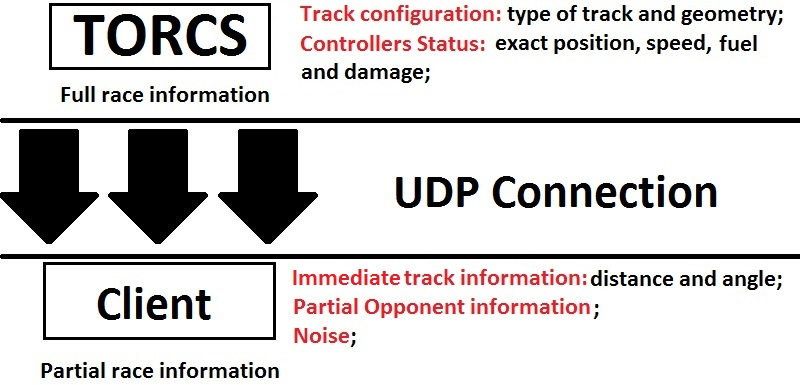
\includegraphics[width=250pt]{Figure1}
		\caption{\label{Fig:1}Available data inside TORCS and at the client.}
	\end{figure}
	
	The complete sensorial input information can be found at the Simulated Car Racing Championship Competition Software Manual~\cite{SCRC}. Noise can be introduced in the sensors, option that is present during the actual competition.

	Race tracks are categorized into \emph{Road}, \emph{Dirt} and \emph{Oval} inside TORCS. The races from the SCRC take place in track types decided by the organization of the championship, information which is not provided to the participants and that may incorporate maps that are unknown to them. The competition adopts a structure that gathers a \textit{Warm-up} stage, a \textit{Qualifier} stage and a \textit{Final} race, which are described in detail in a website of the competition~\cite{SCRC}.
	
	The reason why TORCS presents itself as a satisfactory AI benchmark, in combination with SCRC, is because even	though there are multiple possibilities on how the sensorial input received from the server can be translated into the behavior of the actuators, they can all be compared in a race, which has a robust and steady scoring and evaluational system. In other words, there are many different approaches concerning how to teach the racer encoded by the developers to drive in a racing competition only with the information given by the sensors, and the metric to that issue is the performance on the race itself.

\subsection{Related Works and State of the Art} \label{subsec:Related}
	
	It is very common among some of the SCRC awarded controllers the incorporation of machine learning in their driving methods, along with other evolving techniques using artificial intelligence. As the nature of the problematic presented comprises evolution by experience, learning procedures tend to enhance performance and competitiveness. Essentially, there are two ways of evolving controllers: Online Learning and Offline Learning, the first meaning that improvements are achieved during the actual race execution time and the latter that it is done after it, on the account of the developers themselves and with their own resources by analyzing the data gathered.
	
	The current champion of the SCR Championship is the controller \emph{Mr. Racer}~\cite{MrRacer}, and it has proven to be the State of the Art by winning the last three competitions that happened from 2011 to 2013. The authors of this implementation employ several heuristics and black-box optimization methods in order to reproduce the mechanisms to which human racing drivers resort, doing so by means of a modular structure. \emph{Mr. Racer} uses a Covariance Matrix Adaptation Evolution Strategy (CMA-ES), to evolve parameters offline.
	
	According to the founders of the competition~\cite{SCRC} and the authors of \emph{Mr. Racer} themselves, \emph{AUTOPIA}~\cite{AUTOPIA} is another competitive controller, with the potential to even be the best one available. \emph{AUTOPIA} implements a modular Fuzzy Architecture, whose division contains gear, steering and speed control; and it is optimized by means of a genetic algorithm for Offline Learning, and by means of landmarking the lane exit points for further speed reduction for Online Learning.
	
	These and other controller exemplifications~\cite{SCRC} served as criteria for the analysis and development of the approach presented in this paper. Aspects incorporated and adapted from them feature modularity, offline learning through genetic algorithms, online earning through landmarking and choosing sets of parameters for different categories of tracks, etc. Aspiring to design a controller capable of incorporating these features, the design of a model was proposed and is presented in the succeeding section.
	

	%\section{\textbf{Related Works}} \label{sec:relworks}
	
		The reason why TORCS presents itself as a satisfactory AI benchmark is because there is an infinity of
		possibilities on how the sensorial input received from the server will be translated into the behaviour of the
		actuators, and they can all be compared in a race, which has a robust and steady scoring system. In other
		words, there are many different approaches concerning how to teach the racer encoded by the developers to
		drive in a racing competition only with the information given by the sensors, and the metric to that issue
		is the performance on the race itself.
		
		By controller, let it be understood that the subject is the programming code that in fact controls the
		car/driver/racer within racing environment. Some examples of awarded controllers and their driving methods
		will be presented in this section. They are what can be called the State of the Art among TORCS, and it is
		very common among them the incorporation of machine learning methods, along with other evolving techniques
		using artificial intelligence. Instinctively, as the nature of the problem comprises evolution by experience,
		learning procedures tend to enhance performance and competitiveness. Essentially, there are two ways of
		evolving controllers: Online Learning and Offline Learning, the first meaning that improvements are achieved
		during the actual race execution time and the latter that it is done before the competition, on the account of
		the developers themselves and with their own resources.
		
\subsection{State of the Art}
		
		The current champion of the SCR Championship is the controller \emph{Mr. Racer}~\cite{MrRacer}, and it has
		proven to be the State of the Art by winning at least the last three competitions that happened. The authors
		of this implementation learn parameters offline through Covariance Matrix Adaptation Evolution Strategy
		(CMA-ES), use regression and low-pass filtering to reduce noise impact, distinguish normal asphalted roads
		from dirt-based ones for behavioral separation and implement an authentic opponent-handling method. Their
		Online Learning consists on the track model selection to categorize into dirt or asphalt, choice of databased
		sets of parameters that best fit the track and the tuning of a target speed for all its corners.
		
		Another renowned controller is \emph{AUTOPIA}~\cite{AUTOPIA}. According to the founders of the
		competition~\cite{SoA} and the authors of \emph{Mr. Racer} themselves, it is a competitive match, with the
		potential to even be the best one available, but since no entries were received from them in a while, their
		means of winning a competition were somewhat restrained. Nevertheless, assessing its performance is
		worthwhile, and its description is the implementation of a modular Fuzzy Architecture, whose division contains
		gear, steering and speed control. Their controller is optimized by means of a genetic algorithm for Online
		Learning, and by means of landmarking the lane exit points for further speed reduction for Offline Learning.\toDo{verificar os termos offline e online}
		
		\toDo{Nós vamos	comparar o nosso piloto com o AUTOPIA? Se sim, devemos dizer isso aqui.}
		
		These and other controller exemplifications served as parameters for the analysis and development of the
		approach presented in this paper. Aspects incorporated and adapted feature modularity, offline learning
		through genetic algorithms, online learning through landmarking and choosing sets of parameters for different
		categories of tracks, etc. \toDo{Adicionar o quê mais fizemos no projeto como pincelada inicial para fazer o
		gancho com a seção Controller Structure.}
	\section{\textbf{The FSMDriver}} \label{sec:FSM}
	
	Some of the main aspects discussed to outline a controller for TORCS were sufficed by the concept of finite state
	machines (FSM)~\cite{Millington:2006:FSM}, the most important one being the goal of reaching an autonomous driving
	behaviour in a car race.

	According to Mat Buckland in \emph{Programming Game AI By Example}~\cite{Buckland:2005:AI}:
	
	\begin{quotation}
		
		\emph{
			``A finite state machine is a device, or a model of a device, which has a finite number of states it can be in
			at any given time and can operate on input to either make transitions from one state to another or to cause
			an output or action to take place. A finite state machine can only be in one state at any moment in time.''}
		
	\end{quotation}
	
	This architecture was chosen in order to transform the problem of complex driving into smaller problems of
	situations found within the racing environment, and the division performed for the problematic of this work is
	described in the rest of this section.
	
\subsection{Five-state FSM} \label{subsec:FSM5}
	
	Initially, the design of the finite-state machine proposed comprised the following states:
	
	\begin{itemize}

	\item \emph{Straight Line};
	
	\item \emph{Approaching Curve};
	
	\item \emph{Curve};
	
	\item \emph{Out of Track};
	
	\item \emph{Stuck}.

	\end{itemize}
	
	Essentially, for this method, normal behaviour covered \emph{Straight Line}, \emph{Approaching Curve} and
	\emph{Curve}, as the controller was located inside the track boundaries and no recovery actions needed to be
	considered, whereas exception behaviour consisted of \emph{Out of Track} and \emph{Stuck}, situations in which
	such conduct was expected. Here, a consideration needs to be taken into account: the real first model of the
	finite-state machine did not have an \emph{Approaching Curve} state, but, as the interpretations of the demeanour
	concerning the \emph{Straight Line} and the \emph{Curve} were so different from one another, a preparation had to
	be established so as to smoothen the transitions between them.
	
	If the controller was currently in \emph{Straight Line}, it would be expected of him to simply go as fast as he
	could, with no steering changes whatsoever; when in \emph{Approaching Curve} state, he would reposition himself
	in relation to the track and recalibrate his speed in order to make better curves, which is done by steering the
	car towards the direction of the sensor with the biggest read value and braking until a proportionally calculated
	target speed is achieved; or, when in situations of \emph{Curve}, the pilot would stop braking while maintaining
	the steering direction towards the sensor pointing the biggest distance value read - which represents the
	direction of the curve, prepared by the approaching curve state. For the exception states, even though the
	expected deportment is well known, e.g. a stuck controller should maneuver the car out of the current situation
	and proceed to normal race conduct, the implementations vary among developers. The strategy chosen for the
	exception states was used on both proposals as a matter of regularity of comparison, and is explained on the next
	subsection.
	
	One big problem about this way of treating the matter is that the function responsible for choosing which state
	is more appropriate for each situation would more than often be overcharged, and, in some cases, rather different
	sets of parameters received by it would result in the same classification among the states. Thus, in order to
	minimize the dependency of the driving performance in relation to the function in charge of the transition
	between states, a project decision was made to reduce the number of states.
		
\subsection{Three-State FSM} \label{subsec:FSM3}
	
	\toDo{explicar a inicializacao dos vetores de forma gaussiana}
	The very nature of the initial architecture gave rise to the new approach. As mentioned within this very section,
	three of the states were innately part of a common bigger state, thereby \emph{Straight Line},
	\emph{Approaching Curve} and \emph{Curve} summed into \emph{Inside Track}, resulting in the new controller with
	only three states, which were:
	
	\begin{itemize}
		
		\item \emph{Inside Track};
		
		\item \emph{Out of Track};
		
		\item \emph{Stuck}.
		
	\end{itemize}
	
	\emph{Inside Track}, therefore, is how the car, desirably, will spend most part of the time. The controller
	calculates a \emph{target speed} based on how far the car is from the farthest edge of the track, then, it assumes
	a position of increasing the speed until it reaches this velocity while driving towards the sensor with the
	biggest read value. The distance of this method conveys the greater length the car may advance with little or
	sometimes without significant steer changes This state also brakes, if necessary, when approaching turns.
		
	\emph{Out of Track} is when, for any unknown reason, the car is found outside of the track limits. In this case,
	the proper behaviour is to try to return to the lane. In road tracks, the outside track normally has a different
	terrain, sometimes dirt-based, meaning that skidding frequently occurs, and in an effort to avoid this, a control
	system to brake when the car begins skidding above a threshold was implemented.
	
	\emph{Stuck} represents any given situation that the car is unable to progress in the race. This is a delicate
	state, because it presents itself as difficult to identify and also due to its impact to the performance of the
	controller. In order to detect \emph{Stuck} circumstances, the speed of the car is monitored throughout the race,
	during every game tick, if it lingers with a low speed for a determined period, then it is considered stranded,
	or stuck. When detected, this state activates the reverse gear of the car and turns it until its front is
	directed towards the correct axis of the track. The reason why \emph{Stuck} is a sensitive state is because, when
	detected early, might indicate false positive, and when detected late, could lessen the efficiency of the
	controller. Thusly, detecting \textit{Stuck} situations is crucial, and so is handling the car out of them.
	
	Besides the states, there is also a learning module that is called whenever the \emph{Out of Track} state is
	requested. This module records both speed and position from the state of the car in the vicinity of the departure
	from the track, and retaining these information allows the controller to slow down in subsequent laps when
	approaching the critical points highlighted by the learning module. The implementation of this procedure consists
	on replacing the speed recorded for the landmarked position by a slower one on future occurrences, which is done
	by starting to break in these next occasions. For this work, the module described in this paragraph constitutes
	the Online Learning method, concept introduced in Subsection~\ref{subsec:Related}.
	
	In conclusion, each state in this manner of dealing with the process becomes, ideally, an independent problem,
	whose solution can be attacked separately. This way, they can all have individual sets of parameters susceptible
	to improvement, which will be discussed in the next section.
	
\subsection{Search for Parameter Values - Genetic Algorithm} \label{subsec:GA}
	
	Due to the quantity of parameters to be tuned and the defined granularity, the search space becomes enormous and
	renders fundamental the use of a search algorithm, which optimizes the process of finding better configurations
	by being more incisive and saving resources such as computational time and space. In the present study, an
	evolutionary algorithm was chosen for this task.
	
	A genetic algorithm~\cite{GA} is an evolutionary algorithm inspired by nature, in special by the concept of
	evolution through natural selection~\cite{Darwin}, whose main idea is that a set of solutions for a problem can
	be evolved like the population of a generic species in nature. The applications of genetics algorithms are
	present at many areas, extending from control engineering at non-linear system identification to biomedicine
	prosthesis development and even economy to forecast the behavior of agents.\toDo{referencias sobre aplicacoes}
	
	In this context, a viable solution is called an individual and can be represented by a string of parameters. The
	first population is instantiated randomly to its full extent due to the lack of information concerning how to
	effectively evaluate an individual. This population passes through a fitness function that indexes a score to
	each individual, and this function is responsible for assessing how good - or how adapted - the solution that is
	being evaluate is. After evaluating the population separately, a group of individuals is chosen as the parents of
	the next set of solutions, which will compose a new generation; there are countless ways of performing the
	selection of the parents to the new generation of offspring, and this work gave preference to picking the higher
	individuals on the scoring system, what is called Elitism~\cite{ELITISM}. Each pair of parents is submitted to
	crossover in order to generate two offspring solutions, and in the end of the process each offspring may present
	mutation - everything according to predefined rates. For this work, the crossover takes place in 95\% of the
	reproduction, while the mutation rate assumes the rate of 1\%~\cite{RATES}.
	
	For the Five-state FSM, 22 parameters required adjustment, which originated, in different quantities, from each
	state separately and also the \emph{transition} function, as follows:
	
	\begin{itemize}
		
		\item \emph{Approach Curve} has 4 parameters;
		
		\item \emph{Transition Function} has 3 parameters;
		
		\item \emph{Straight Line} has 4 parameters;
		
		\item \emph{Out of Track} has 7 parameters;
		
		\item \emph{Stuck} has 4 parameters.
		
	\end{itemize}
	
	However, for the Three-state FSM, only 19 parameters demanded adjustment, which are divided as follows:
	
	\begin{itemize}
		
		\item \emph{Inside Track} has 8 parameters;
		
		\item \emph{Out of Track} has 7 parameters;
		
		\item \emph{Stuck} has 4 parameters.
		
	\end{itemize}
	
	Theoretically, as the search space for the latter case is smaller, finding a better controller was expected to
	happen first for it, but only by effectively testing both architectures could such a result be achieved. The
	source codes for both models presented in this section are available at the \emph{GitHub} repository provided in
	the references~\cite{GitHub}.
	
	%\section{Genetic Algorithm}
	Due to the quantity of parameters to be tuned and the defined granularity, the space search is enormous and it's necessary some space search algorithm. In this study was chosen a evolutionary algorithm.
	
	
	A genetic algorithms are adaptive heuristic search algorithm based on the evolutionary ideas of natural selection. Genetics algorithms applications are present at many areas such as control engineering at non-linear system identification, biomedics to develop legs mechanism to proteses and even economy to forecast the behavior of agents.  
	
	Each individual is a string that contain the information necessary to evaluation. Usually, the values that composes the strings are parameters to be tuned. The search space of the optimization of parameters is defined by the representation of the chromosome.
		
	
	A randomly initial population is created, than, accordingly with the fitness function, is associated a score for each individual that represents how good the individual is.	
	
	
	Based on the premise that the better ones is more likely to reproduce a better offspring than others, the parents are chosen by the score of each individual. Thus your genetic material can be spread.
	
	
	To increase a genetic diversity each chromosome has a tiny chance to be mutate, this avoid a fast convergence of the algorithm, trying not to be stuck in a maximum local.
	
	
	For the model with 5 states, it was necessary adjust 22 parameters, each state has a different quantity, including the \emph{transition} function, as follows:

	\emph{Approach Curve} has 4 parameters.

	\emph{Transition Function} has 3 parameters.

	\emph{Straight Line} has 4 parameters.

	\emph{Out of Track} has 7 parameters.

	\emph{Stuck} has 4 parameters.
	
	
	

	\section{Experimental Results} \label{sec:Experiments}

	A veil was put over the Five-state FSM from the very beginning of the experimentation phase, which was its great dependency towards the transition function. Early superficial evaluations of the performance of this first model indicated an overcharge concerning this function, which was verified by considerable changes in behaviour derived from adjustments in its parameters. For that reason, a second model with less states - the Three-state FSM - was designed regarding this characteristic and releasing part of the performance burden from the transition function, and the results from the comparison of these architectures are described and analyzed in the succeeding subsections.

\subsection{Methodology} \label{subsec:Methodology}

	Once the models - and which of their parameters required tuning - had been defined, the genetic algorithm was applied to each approach separately, in order to adjust their configurations for superior and competitive status. At the same time, the goal was to find general and versatile controllers with good results for any track and specific ones that were fittest to race in various tracks: road, dirt and oval alike. Therefore, due to the differences observed in the parameters of controllers evolved on dirt and road tracks, the evolution process took place separately for those two kinds of environments, which produced two contrasting sets of enhanced values for each model.
	
	The \emph{metric} chosen to evaluate the generated controllers was the combined sum of the distance raced by the car alone in the first 10 000 game cycles - also called \emph{game tics} - in a list of mixed tracks. This value will henceforth be called the \emph{fitness} of the controller, as it was used to determine whether he would remain in the evolution process.
	
	The experiments concerning Oval Tracks would repeatedly provide inconclusive results, so they were neglected in this evaluation process. Thus, in order to find the best set of parameters for a general track, the two finite-state states were evolved in three different sets of tracks, one with 4 Dirt Tracks, one with 4 Road Tracks and another with the 4 of each type. The evolution process for each set of tracks consisted on 600 generations of 30 individuals and culminated in one controller; in other words, at the end of the experiments, there were six evolved controllers, one specific for Road Tracks for each model, one specific for Dirt Tracks for each model, and also one evolved in a mixed manner for each model. Additionally, as the \emph{Stuck State} is only triggered in very specific situations, it was not evolved with the controller and its parameters were hand tuned.
	
	Pursuing an unbiased choice of parameters, the Online Learning module described in Subsection~\ref{subsec:FSM3} was turned off during the evolution progress as it seizes the responsibility for the behaviour of the car for itself during the race and could interfere with natural selection. The validation then occurred through testing the six produced pilots in a predefined set of tracks different from those in which they were evolved, avoiding the evidence of too track-limited parameters. On behalf of comparison, the results from the AUTOPIA controller were incorporated in the analysis, since it can be considered the State of the Art, displaying one of the best performances for the SCR Championship, and should provide satisfactory basis for appraisal.

	The four Road Tracks used in the evolution process were chosen from the TORCS standard track set, which are \emph{Spring}, the longest track available on TORCS with more curves than any other track, \emph{Wheel 2}, the most difficult track with sharp and hard curves, \emph{E-Track 3}, a fast track with turns that put to test the dexterity of the controller, and \emph{Forza}, a track considered to be raced fast and whose curve pattern is usually found in others tracks. Also four Dirt Tracks were selected to be used in evolution, which were \emph{Dirt2}, \emph{Mixed1}, \emph{Mixed2}, \emph{Dirt6}. \emph{Dirt2} is a difficult track with close curves, while \emph{Mixed1} is an easy one with few curves, also, \emph{Mixed2} has many turns with medium difficulty, and \emph{Dirt6} present hard curves.
	
	Once the evolution process was finished, the six resultant controllers were tested in the evaluation set of tracks, different from those where they were evolved. Three Road Tracks were picked to evaluate the controllers, they are also available on TORCS and were used both in the competitions of 2008 and to evaluate the \emph{AUTOPIA} controller~\cite{AUTOPIA2009}. \emph{Street-1} and \emph{D-Speedway} were used at the \emph{IEEE World Congress on Computational Intelligence}; and \emph{CG Speedway 1} was used at the \emph{Computational Intelligence and Games Symposium - CIG}. This set also contained three Dirt Tracks, which were \emph{Dirt1}, \emph{Dirt3}, \emph{Dirt4}. \emph{Dirt1} has smooth curves and allows the controller to perform in high speed, while \emph{Dirt3} is an easy one with few curves, also, \emph{Dirt4} has many turns with medium difficulty and is the longest Dirt Track available.
	  
	
\subsection{Results} \label{subsec:Results}
	
	It is important to mention that before each result displayed in that section a warm-up stage was held for 5 laps in each track.
	
	The controllers were submitted to a set of evaluation races and the distances they covered in 10 000 game tics inside each of those races were joined in Table~\ref{tbl:dist covered}. This table also displays how the evolved controllers performed in comparison to the AUTOPIA controller.
	
	In order to have a more in-depth comparison, Table~\ref{tbl:time raced} was assembled to display the time elapsed during 10 laps for each of the previous tracks tested. The \textit{Berniw Hist4} bot provided by the TORCS distribution was also used in this test phase even though it uses a different car from those allowed in the SCRC~\cite{2009} and has a low performance compared to the others bots provided. AUTOPIA also uses this bot for comparison~\cite{AUTOPIA}.
	
	\begin{table*}[t]
	\renewcommand{\arraystretch}{1.3}
	\caption{Distance covered in meters racing alone for 10 000 game tics}
	\label{tbl:dist covered}
	\centering
	\begin{tabular}{c||c||c||c||c||c||c}
	\hline
	\bfseries Driver & \bfseries Street-1 & \bfseries D-speedway & \bfseries CG-speedway & \bfseries Dirt-1 & \bfseries Dirt-3 & \bfseries Dirt-4 \\ 
	\hline	
	\hline FSM3(road) & \textbf{7925.6} & 13196.5 & 8745.49 & 3978.01 & 3451.26 & 6757.83 \\
	\hline FSM3(dirt) & 2149.77	& 2450.84 & 1951.93	& 3525.84 & 4905.58 & 5590.78 \\
	\hline FSM3(mixed) & 7219.28 & 12772.4 & 8126.12 & \textbf{4386.64} & \textbf{5481.15} & \textbf{6939.83} \\
	\hline FSM5(road) & 3822.76 & 3427.11 & 4114.66	& 2145.49 &	2205.97 & 3260.19 \\
	\hline FSM5(dirt) & 1267.83 & 2936.82 &	4114.66 & 1072.92 &	2205.82 & 3260.33 \\
	\hline FSM5(mixed) & 3822.99 & 3427.06 & 4114.8 & 2145.75 &	2205.83 & 3260.31 \\
	\hline AUTOPIA & 7091.8 & \textbf{15612.3} & \textbf{8970.4} & * & * & * \\
	\hline 
	\end{tabular} 
	\end{table*}

	
	\begin{table*}[t]
	\renewcommand{\arraystretch}{1.3}
	\caption{Time elapsed in seconds racing alone for 10 laps}
	\label{tbl:time raced}
	\centering
	\begin{tabular}{c||c||c||c||c||c||c}
	\hline
	\bfseries Driver & \bfseries Street-1 & \bfseries D-speedway & \bfseries CG-speedway & \bfseries Dirt-1 & \bfseries Dirt-3 & \bfseries Dirt-4 \\ 
	\hline
		\hline FSM3(road) & \textbf{1086.3} & 607.4 & \textbf{495.0} & \textdagger & 1150.1 & 1756.4 \\
	\hline FSM3(dirt) & \textdagger & 840.0 & 1274.8 & 597.3 & 1089.4 & 1307.5 \\
	\hline FSM3(mixed) & 1216.50 & \textbf{572.60} & 613.77& 530.0 & 842.9 & 1005.9 \\
	\hline FSM5(road) & \textdagger & \textdagger & 816.6 & \textdagger & \textdagger & \textdagger \\
	\hline FSM5(dirt) & \textdagger & \textdagger & \textdagger & \textdagger &	\textdagger & \textdagger \\
	\hline FSM5(mixed) & \textdagger & \textdagger & \textdagger & \textdagger & \textdagger & \textdagger \\
	\hline Berniw Hist4 Bot & 1143.77 & 656.24 & 605.76 & 460.95 & 872.97 & 1127.45 \\
	\hline AUTOPIA & * & * & * & \textbf{339.3} & \textbf{742.4} & \textbf{796.5} \\
	\hline 
	\end{tabular} 
	\end{table*}
	
	It is important to mention that the bots have a full view of the track format and do not use the sensors provided by SCR. Instead, they have directly access to all the information necessary to race, which gives them some advantage over the controllers developed for the TORCS environment, such as the ones described in this paper, which receive only the information that comes from sensors and in addition have to interpret them in order to abstract how the track really is. 
	
\subsection{Analysis} \label{subsec:Analysis}
	
	The best pilots from each race evaluated by Tables~\ref{tbl:dist covered} and~\ref{tbl:time raced} were highlighted in bold. Both sets of experimental results shown at these tables were selected in order to match previous tests performed by the AUTOPIA controller. In 2009, the authors of AUTOPIA~\cite{AUTOPIA2009} evaluated it through racing for a predefined time period and computing the total distance reached, and these results were incorporated in Table~\ref{tbl:dist covered} for comparison. Differently, in 2012, this controller~\cite{AUTOPIA} was assessed by racing alone during 10 laps and calculating the time elapsed to do so, and these results were also incorporated in the evaluation process of this paper and are displayed in Table~\ref{tbl:time raced}. The tracks that are not present in either of the tests executed by AUTOPIA were validated only between the approaches proposed by this paper, which was informed in Tables~\ref{tbl:dist covered} and~\ref{tbl:time raced} through the ``*'' symbol, meaning that AUTOPIA had no results for that race in particular.
	
	For a wider analysis not only the numeric results were taken into account in this section but also observations made in the graphic mode provided by the TORCS distribution.
\subsubsection{Comparing the Controllers Proposed} \label{subsubsec:CompControllers}
	
	The overall comparison between the two approaches presented favored the Three-State FSM, on account of the considerably superior results it produced in all the tracks tested. The Five-State FSM presents a very complex transition function that takes into account the variance of the sensorial input to decide if the car is in a straight line, approaching a turn or in a turn. On the other hand, the Three-State FSM has only a single state for handling normal driving situations and it is very easy to say if the controller is inside or outside the track only by checking the track sensor. This contrast in behavior is then interpreted to be the reason of the overwhelming difference in performance, the complexity of the transition function, which supports the initial hypothesis of the evaluation. Due to this attribute, the Five-State FSM undergoes a lot of damage in its car, which can be noted in Table~\ref{tbl:time raced} where all the ``\textdagger'' symbols represent individuals that did not finish the race for the reason of reaching the maximum damage permitted.
	
	Because the Three-State FSM demonstrated better results than the other approach proposed, it was elected to be subject of analysis on the evaluation process. As expected, the controller evolved only on Road Tracks was the fastest one. These tracks provide an environment susceptible to high speeds, since its curves are smoother and the friction experienced by the car is higher than the ones from Dirt Tracks. These factors, when combined, allow the controller to race without having to steer too abruptly and to brake without losing control while racing in Road Tracks. Consequently, as the friction increases, steering becomes more accurate in road tracks, practically eliminating critical skidding. Therefore, the result from this end of the evolution process was an aggressive driver with high base-speed.
	
	Dirt Tracks provide a more difficult environment for the pilot to fit in. Sudden braking in tracks of this type often results in unwanted behavior, skidding is noticeably more common then. The driver evolved in this end of the evolution process tends to drive in a low speed so it can keep itself inside the boundaries of the track. Speed driving results in higher damage outcomes and even in the total loss of the car in critical situations. The result obtained was a very careful driver with a low base-speed, and an early brake policy - the car starting to brake far before the turn. This passive driving pattern obtained the smallest distance covered both for the Three-State and the Five-State FSMs.
	
	The driver evolved in a mixed set of tracks combines characteristics from both of them. It drives in a reasonable speed comparing to the first one, but also has the preventive brake policy from the second one. This last end of the evolution process achieved better results than the dirt-evolved behavior in all the tracks tested and outperformed the road-evolved one in every single dirt track. From this information gathered, it was inferred that the controller evolved in mixed tracks tries to reach higher speeds even though this means leaving the track in some turns, mostly because the time spent trying to get back to the racing lane is compensated by the speed of the car. The aggressive behavior inherited from the road-evolved end of the evolution makes this latest controller receive ample damage when leaving the track, and also causes it to hit walls, which resulted in the premature ending of some of the tested races, due to reaching the maximum acceptable damage.
	
\subsubsection{Comparing the Three-State FSM to AUTOPIA} \label{subsubsec:CompAUTOPIA}

	Once the Three-State FSM was demonstrated to be more suitable to competitive environments due to its superior performance regarding the Five-State FSM, it was compared to the renowned controller AUTOPIA. Using the distance covered after racing alone in Road Tracks for 10 000 game tics as metric, the Three-State FSMs evolved in Road Tracks and in mixed tracks were able to overcome AUTOPIA in 1 of the 3 tracks tested, as displayed in the bold values in Table~\ref{tbl:dist covered}. The road-evolved Three-State FSM was the controller that got closer to this State of the Art approach using the ``distance raced'', which comes to endorse the assumption of it being a competitive proposal.
	
	However, while racing alone for 10 laps and computing the time elapsed as metric, AUTOPIA outperformed every controller proposed, just as can be seen in Table~\ref{tbl:time raced}. Even though the Three-State controller with Road evolved parameters outperformed AUTOPIA in the first 10 000 tics it was not capable of maintaining the advantage in longer races. As the road evolved pilot presents a more aggressive behavior even though it means taking more damage it has a gain in performance for the early stages of the race. Although when racing for more than a couple laps the controller becomes more careful after each lap reducing it speed to maintain itself inside the track.
	
	The online learning module plays a crucial role in the overall controller's performance as it prevents unwanted situations to repeat, for example leaving the track. Although this strong dependence might result in performance loss as the controller will gradually reduces it speed after each lap in those points where it leaves the track. More accurate actuators control may reduce the dependence of this module and therefore improves performance.
	
	These results can be used to infer that the Five-State and the Three-State FSMs have a great deal of improvement to achieve when it comes to endurance. The Five-State FSM received total loss and did not complete almost every test performed, ending only one race using this metric. The Three-State FSM, on the other hand, completed practically all the tracks, but did not surpass AUTOPIA in either of them. In order to enhance the endurance feature in the controllers proposed, more robust behavior concerning situations in which the car might crash must be taken into account.	
	
	
	\section{Conclusions} \label{sec:Conclusions}

	This paper proposed two approaches developed to control a car during a race in a simulated computational environment, the game platform TORCS. The models of both of these controllers were described, explained, enhanced by means of a genetic algorithm, compared and then tested together with a State of the Art controller - AUTOPIA. It was implied before the testing phase that a finite state machine too burdened in the process of transition between states might lose performance, which was corroborated by the experimental results of the comparison of the two models detailed.
		
\subsection{Conclusions} \label{subsec:Conclusions}

	The finite state machine with less states achieved a superior overall performance in the tests carried out, in relation to the one with more states. The simplifications fashioned in the transition function of the former were inferred to be the reason for this improvement, along with its intricate relation with the number of parameters that were target of fine tuning in the evaluation and validation process.
	
	The evolution procedure adopted concerning the controllers culminated in three characteristic behaviors. The controller evolved on road tracks became a fast driver, whose hastiness resulted in a careless attitude in general; in other words, it was only good for races in road tracks. The one evolved on dirt tracks turned out to be too careful in contrast, limitedly determining its speeds and, in efficiency terms, inferior. The controller evolved on a mixed set of tracks inherited characteristics from both the previous ones, becoming swift but not too hasty, prudent but not too slow. The latter surpassed the performance of the dirt-evolved drivers even on dirt tracks, and did not lose by far on road tracks in comparison to drivers evolved solely in them.
	
	In terms of speed, the Three-State FSM was able to overcome AUTOPIA in one of the three tracks used to validate the drivers using the distance covered in 10 000 game tics as metric. However, in comparison to the same controller, using the time elapsed to race 10 laps as metric instead, the experimental results provided an insight on the lack of endurance that the finite state machine drivers proposed possess.
	
	To sum up, the interpretation of the global results from the experiments performed gives margin to declare that finite state machines are a reliable technique to implement artificial intelligences, at least for computer games such as simulated races. They provide the possibility of parallel development and also enable parameter tuning in separate fronts, due to the independence and abstraction between the behaviors from each state. Finite state machines also represent a valuable tool for describing an operation model for a process, simplifying and gathering possible situations it might present into straightforward categories of accessible understanding.

\subsection{Future Works} \label{subsec:Future}
	
	One characteristic that has been marked as a deficiency in the controllers presented in this paper is the lack of endurance. In order to prevent this from affecting the general performance of the controllers developed, more robust techniques must be integrated into their model. Ways of treating this matter range from harsher brake policies to drive planning intensification, which are already being taken into account for future proposals.
		
	Another important task to be accomplished is the opponent treatment in real-time races. Routines to reduce collisions, i.e., avoiding being overtaken and also being concerned about overtaking the opponents is a fundamental issue. Ignoring adjacent cars usually causes the driver to face unexpected collisions, ending up stuck, considering a worst case scenario. Many of the renowned developers for TORCS already incorporate such treatment in their controllers, and neglecting this necessity renders any driver less robust to unexpected race events, and also reduces its performance.
	
	
	%\section{Future Works} 	
	\begin{itemize}
		 \item Since at the SCRC the controller is allowed to perform a warm-up before the race it is possible to acquire the track data, not only mapping critical section such as sharp curves and points where the car go out the track to improve the result of the controller at the race itself. Also a warp-up stage would supply the information about environment where the car is, including the type of track,road or dirt, which determine a set of parameters best fitted to which occasion. 
        
		\item One important task to be accomplish is the opponent treatment, routines to reduce collisions, avoid the controller to be surpassed and surpass the opponents is a fundamental issue. Ignoring the opponent would make the driver to face unexpected collisions ending stuck, considering the worst event.
	\end{itemize}
	

	


	%\section*{Acknowledgements}

	\bibliographystyle{sbgames}
	\bibliography{Bibliography}

\end{document}
